\documentclass[11pt]{beamer}
\usepackage[utf8]{inputenc}
\usepackage[T1]{fontenc}
\usepackage{lmodern}
\usepackage[spanish]{babel}
\usetheme{EastLansing}
 \usepackage{graphicx}
\usepackage{tikz}
\usetikzlibrary{shapes.geometric, arrows}

\author{Dr. Alejandro Rodriguez}
\title{Probabilidad y Estad\'istica}
\subtitle{Universidad Tecnol\'ogica Iz\'ucar de Matamoros\\UTIM }
%\logo{}
%\institute{}
%\date{}
%\subject{}
%\setbeamercovered{transparent}
%\setbeamertemplate{navigation symbols}{}
\begin{document}
  \begin{frame}[plain]
    \maketitle
  \end{frame}
  \section{Introducción a la asignatura}
    \begin{frame}
      \begin{enumerate}
        \item Estadística Descriptiva
        \item Probabilidad
        \item Estadística Inferencial
      \end{enumerate}
    \end{frame}

    \begin{frame}{Definiciones importantes}

      \begin{block}{Estad\'istica}
        Es un conjunto de procedimientos que sirven para organizar y resumir datos, hacer inferencias a partir de ellos y transmitir los resultados de manera clara, concisa y significativa.
      \end{block}
      \pause
      \begin{block}{Estadística Descriptiva}
        Es un conjunto de procedimientos que sirven para organizar, describir y sintetizar datos, sin que las conclusiones que se extraigan de \'estos rebasen su \'ambito     específico.
      \end{block}


      \footnotetext[1]{Cada definici\'on ser\'a enriquecida m\'as adelante.}
    \end{frame}

    \begin{frame}{Definiciones importantes}

        \begin{block}{Probabilidad}
            El término probabilidad se refiere al estudio de azar y la incertidumbre en cualquier situación en la cual varios posibles sucesos pueden ocurrir; la disciplina de la probabilidad proporciona métodos de cuantificar las oportunidades y probabilidades asociadas con varios sucesos planeado o en una investigación científica.
        \end{block}
        \pause
        \begin{block}{Estadística Inferencial}
          Es un conjunto de procedimientos que se emplean para hacer inferencias y  generalizaciones respecto a una totalidad, partiendo del estudio de un n\'umero limitado de casos tomados de esta \'ultima.
        \end{block}

        \footnotetext[1]{Cada definición será enriquecida más adelante.}
    \end{frame}

    \begin{frame}

    \end{frame}

  \section{Estadística Descriptiva}

    \begin{frame}
      \textbf{\begin{center}
      \huge Estadística Descriptiva
      \end{center}}
    \end{frame}

    \begin{frame}{Estadística Descriptiva}
      \begin{block}{Estadística Descriptiva}
          Es un conjunto de procedimientos que sirven para organizar, describir y sintetizar datos, sin que las conclusiones que se extraigan de \'estos rebasen su \'ambito     específico.
      \end{block}
    \end{frame}


    \begin{frame}
      \begin{block}{Ejemplo A}
        \begin{figure}
            \centering
            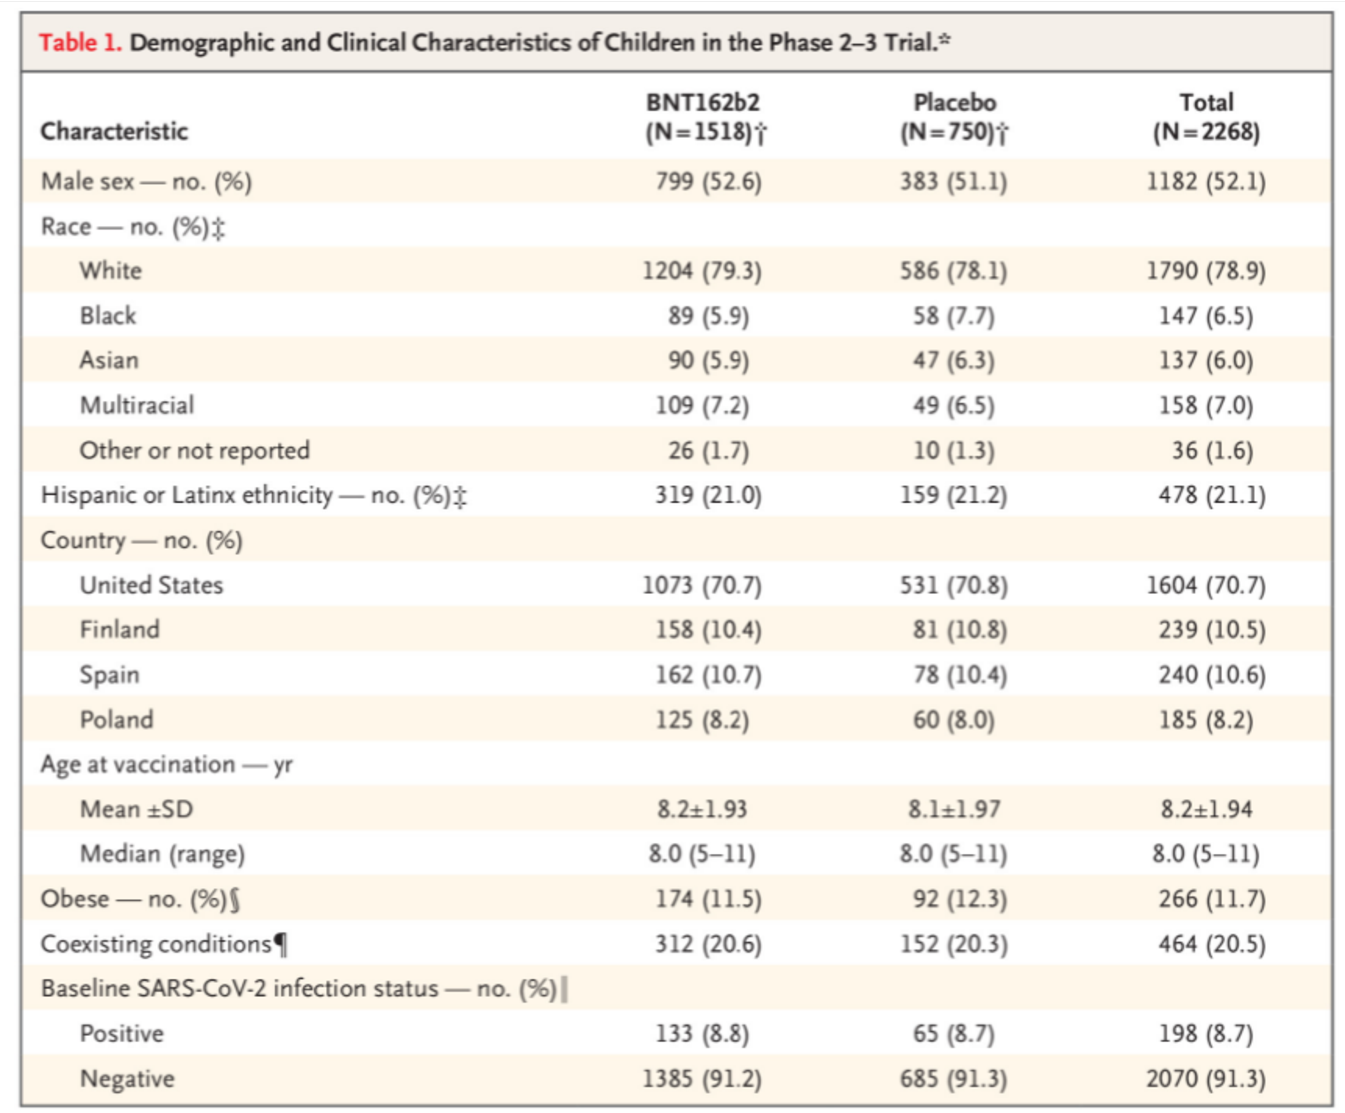
\includegraphics[width=0.7\linewidth]{images/Lecture_1a}
            \label{fig:lecture1a}
        \end{figure}
      \end{block}
    \end{frame}
    \begin{frame}
      \begin{block}{Ejemplo B}
        \begin{figure}
            \centering
            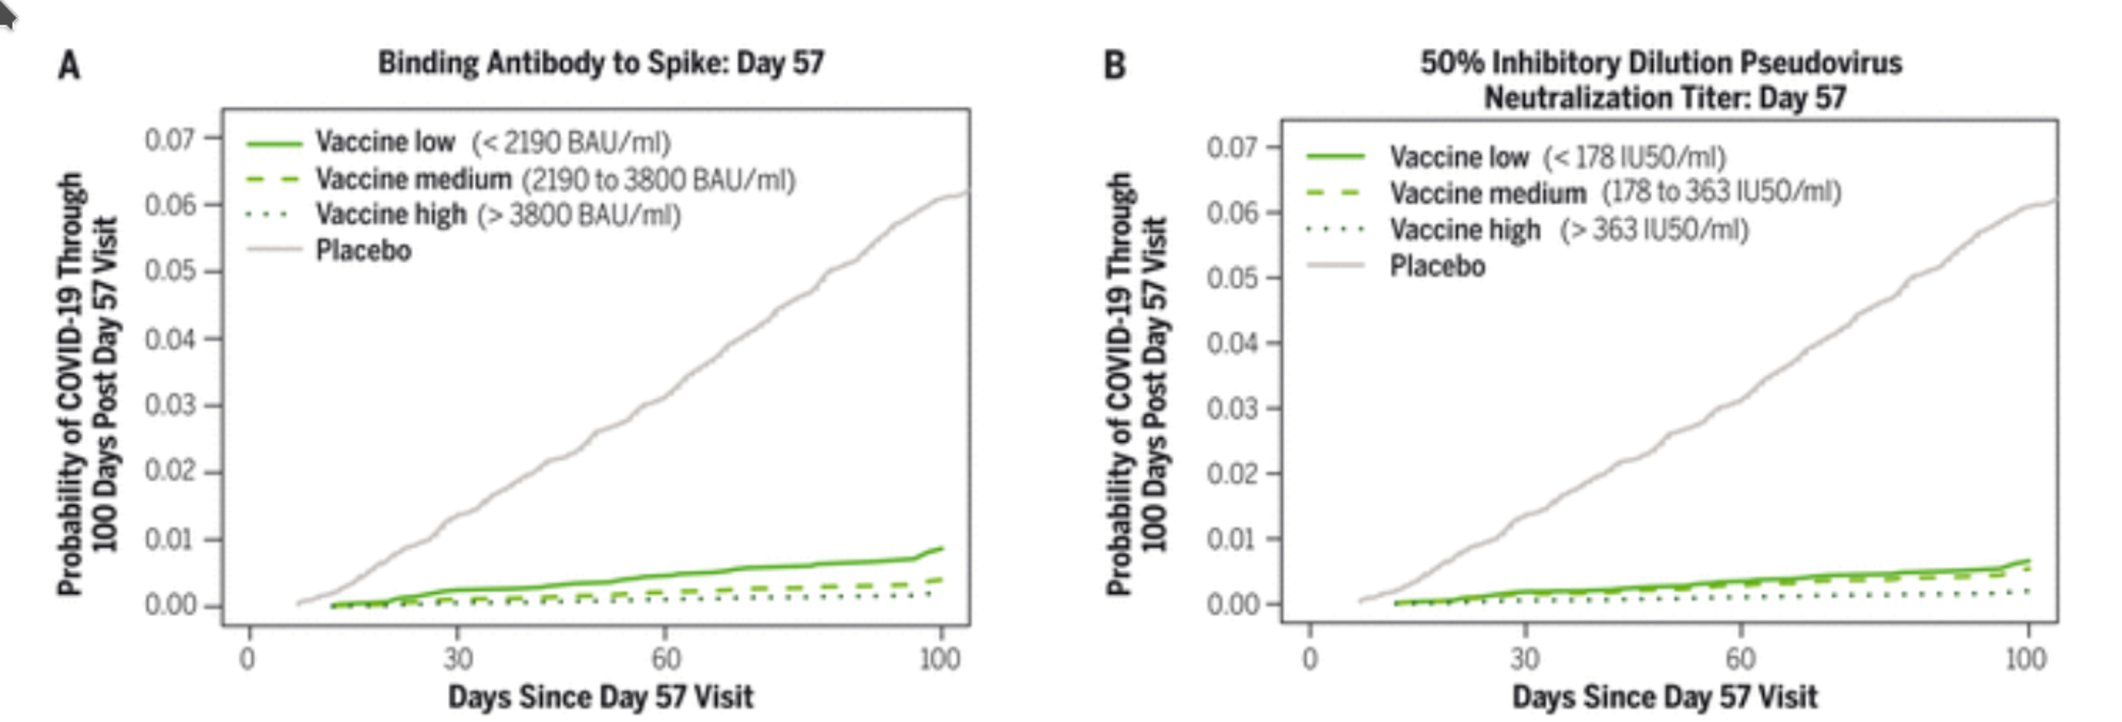
\includegraphics[width=1\linewidth]{images/Lecture_1b}
            \label{fig:lecture1b}
        \end{figure}
      \end{block}
    \end{frame}

    \subsection{Variable estadística}
    \begin{frame}{Variable estadística}
      \begin{block}{Variable estadística}
         Variable es cualquier característica cuyo valor puede cambiar de un objeto a otro en la población objeto de estudio. Estos valores a su vez se caracterizan por poder ser medidos.
      \end{block}

    \end{frame}

    \begin{frame}{Variables}
      \begin{figure}
        \centering
        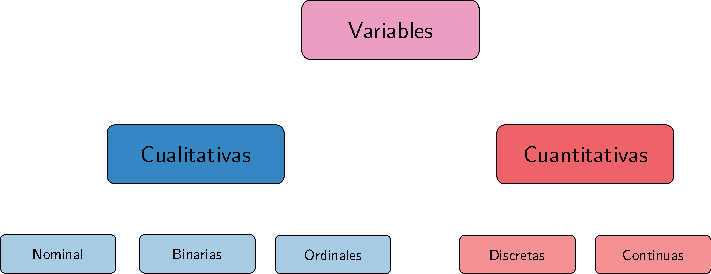
\includegraphics[width=1\linewidth]{images/Lecture_1c}
        \label{fig:variables}
      \end{figure}
      \pause
      Un estudio de una sola variable se conoce como datos \textbf{\textit{univariante}}.De igual forma si se hace un estudio donde varían dos variables se le llama \textit{\textbf{bivariante}}.
    \end{frame}

    \begin{frame}{Ejemplo de variables}
        \centering
        \begin{tabular}{|c|c|c|c|c|c|}
            \hline
            Id & Nombre & Peso & Escolaridad & Alergia & Localidad \\
            \hline
            1 & Richard Feynman & 80.6Kg & PhD & No & NY City \\
            \hline
            2 & Yuri Gagarin  & 95.3Kg & Coronel & SI & Smolensk  \\
            \hline
            3 & Manuel Mercado & 70.0Kg & Licenciado & NO  & C. de México \\
            \hline
            C.D & C.N  & C.D & C.O & C.B & C.N \\
            \hline
        \end{tabular}
    \end{frame}


    \subsection{Población, Muestra y Muestreo}
    \begin{frame}
        \centering
        \textbf{\huge Población, Muestra y Elemento}
    \end{frame}
    \begin{frame}{Población, Muestra, Elemento}
        \begin{block}{Población}
            La \textit{\textbf{población}} o también llamada \textbf{\textit{universo}}, es todo conjunto de personas, cosas u objetos con ciertas características comunes sujetos a un estudio en cuestión.
        \end{block}
        \pause
        \begin{block}{Muestra}
            Definida una población cualquiera, se llama \textit{\textbf{muestra}} a toda porción de elementos sacada de ella.
        \end{block}
        \pause
        \begin{block}{Elemento o Unidad}
            Cada uno de los componentes de una población recibe el nombre de \textit{\textbf{elemento}} o \textbf{unidad} esencial.
        \end{block}
    \end{frame}
    \begin{frame}{}
        \begin{figure}
            \centering
            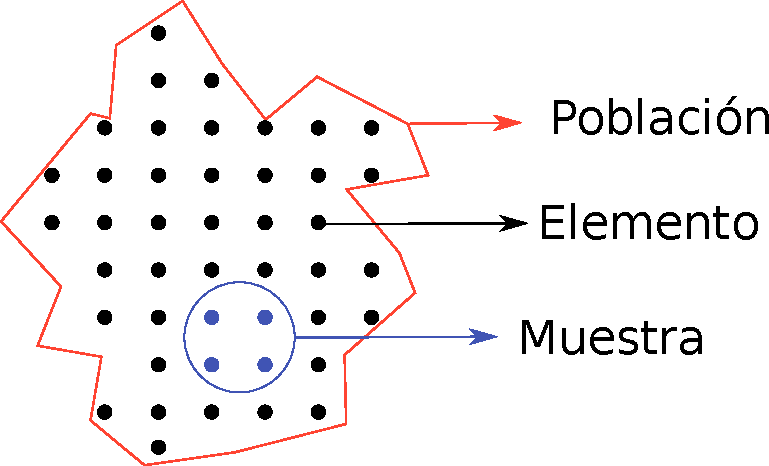
\includegraphics[width=0.9\linewidth]{images/Lecture_1d}
            \label{fig:lecture1d}
        \end{figure}
    \end{frame}
    \begin{frame}{}
      \begin{figure}
        \centering
          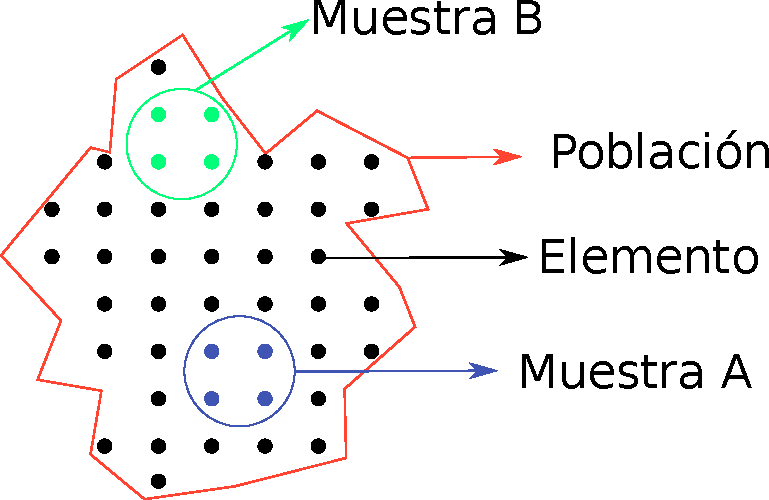
\includegraphics[width=0.9\linewidth]{images/Lecture_1e}
        \label{fig:lecture1e}
      \end{figure}
    \end{frame}
    \begin{frame}{}
      \begin{figure}
        \centering
        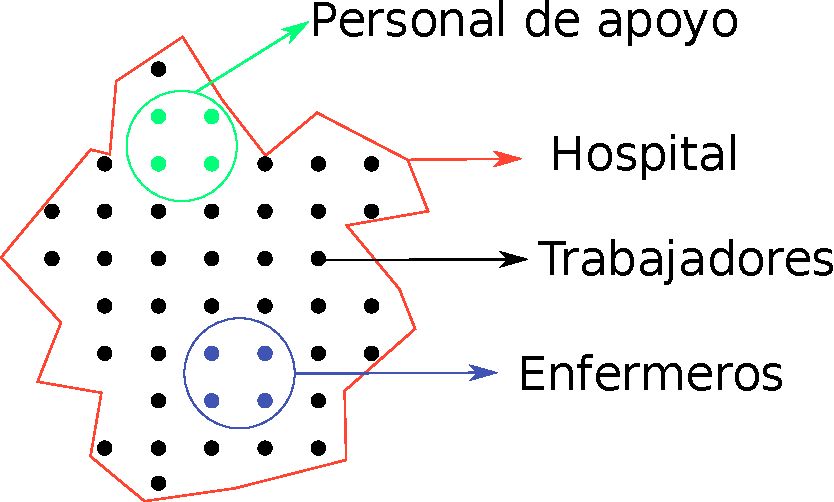
\includegraphics[width=0.9\linewidth]{images/Lecture_1f}
        \label{fig:lecture1f}
      \end{figure}
    \end{frame}

    \begin{frame}{Tarea}
        \begin{block}{Tarea 1}
            \begin{figure}
                \centering
                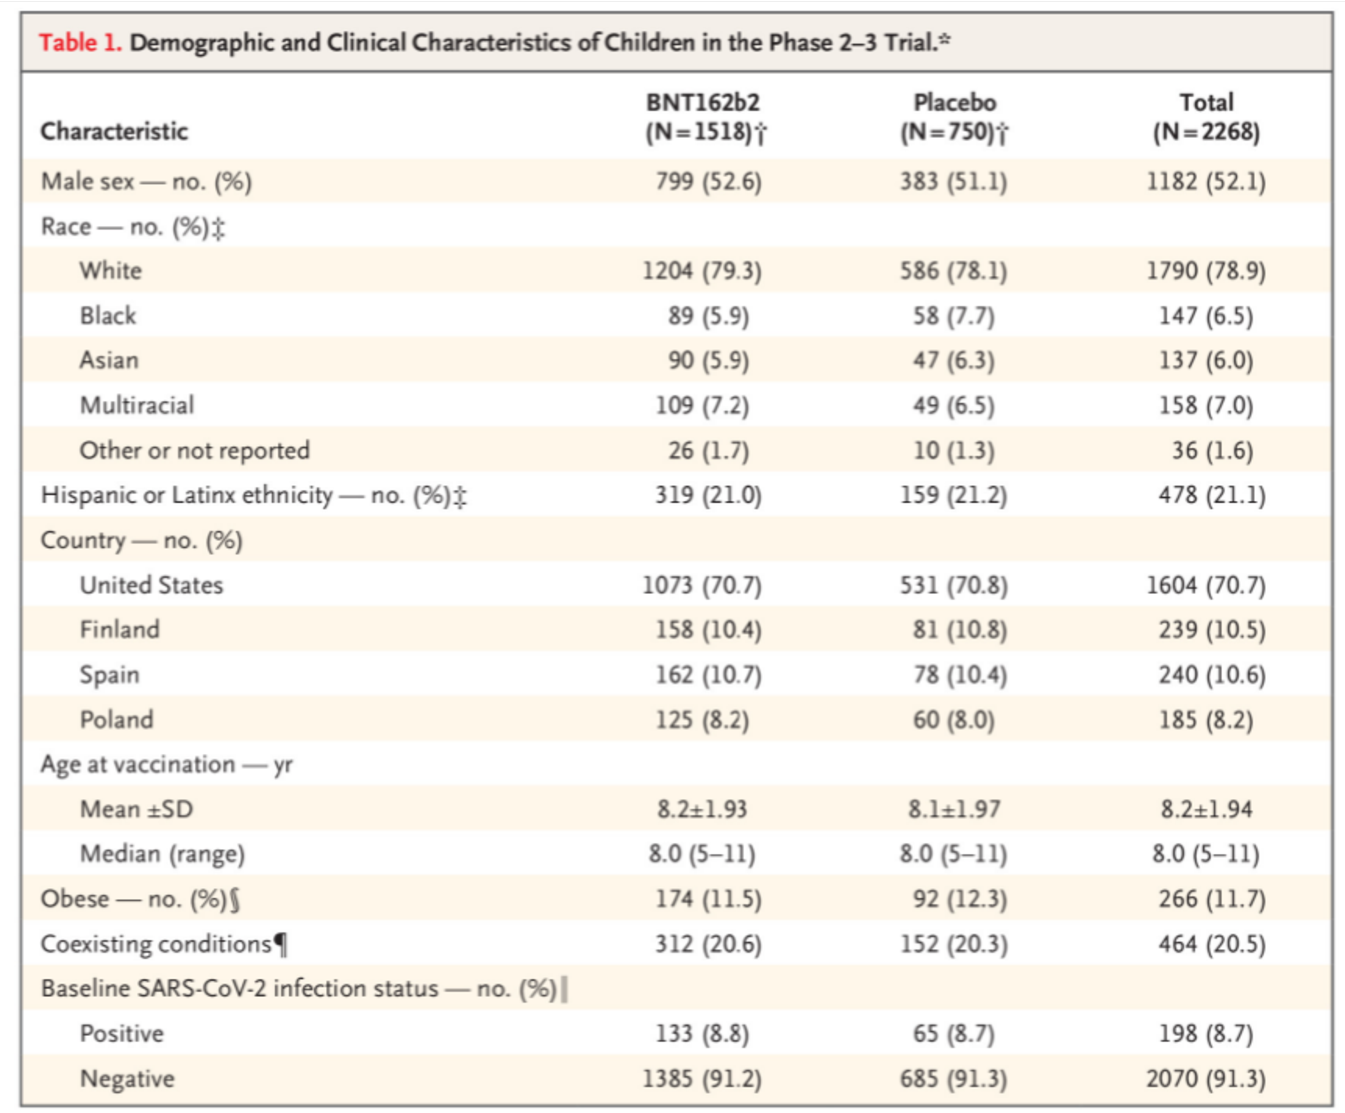
\includegraphics[width=0.7\linewidth]{images/Lecture_1a}
                \label{fig:lecture1aa}
            \end{figure}
        \end{block}
       \textbf{ Identifique:} Población, Muestra y elemento
    \end{frame}
    \begin{frame}{Tarea}
        \begin{block}{Tarea 2}
            \begin{figure}
                \centering
                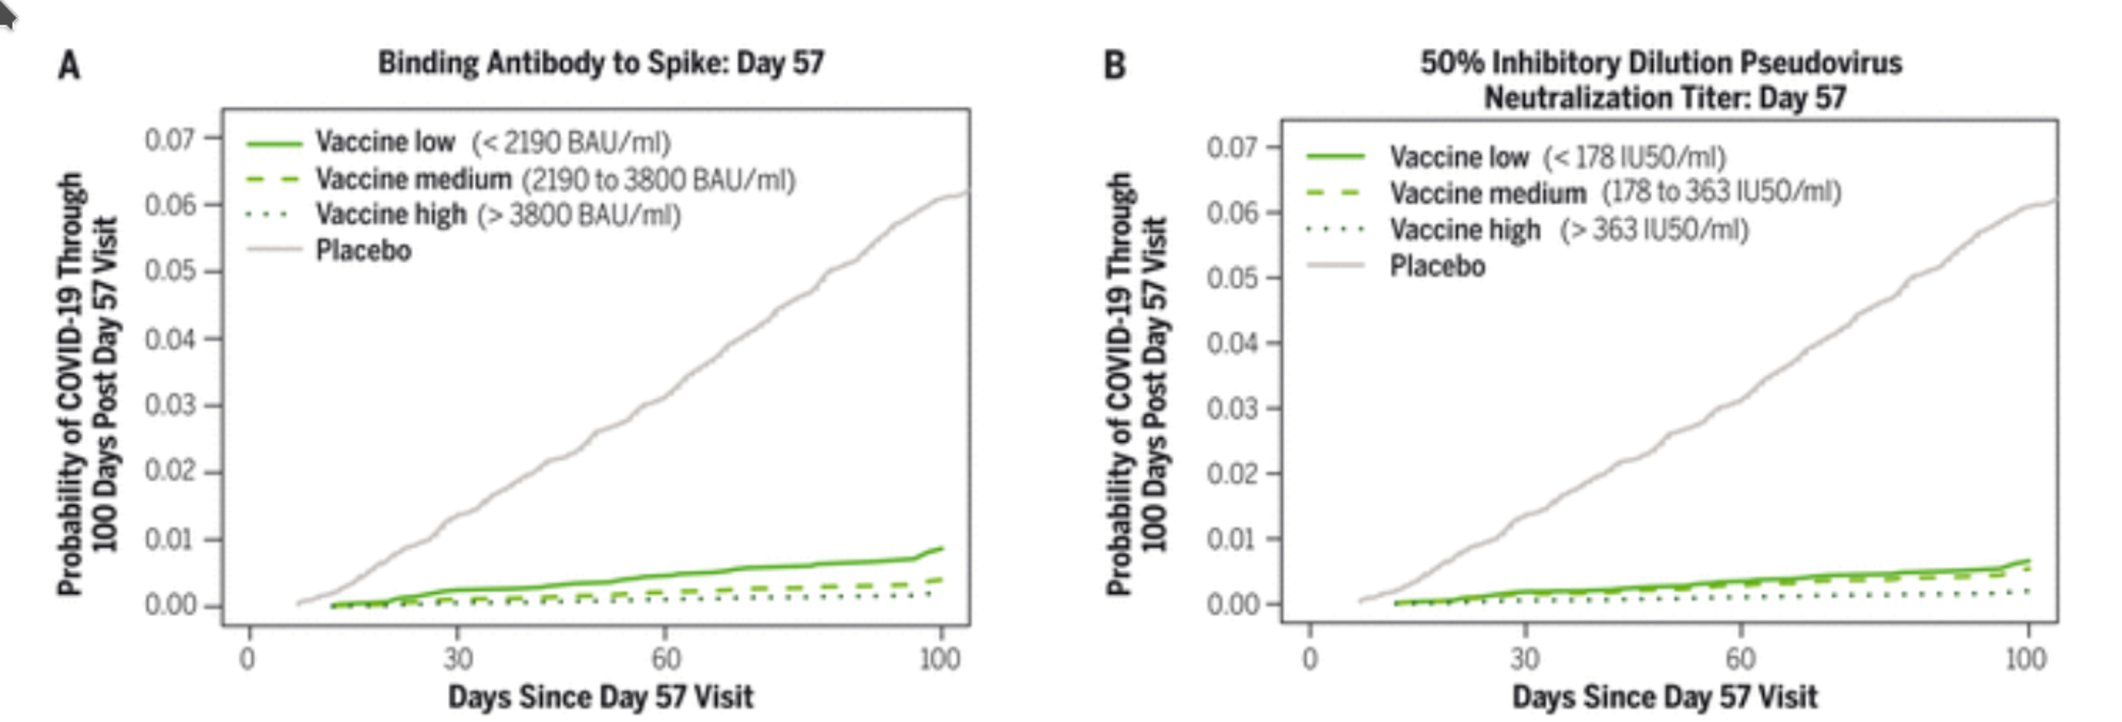
\includegraphics[width=1\linewidth]{images/Lecture_1b}
                \label{fig:lecture1bb}
            \end{figure}
        \end{block}
        \textbf{Identifique:} Población, Muestra y elemento
    \end{frame}

    \begin{frame}{}
      \centering
      \begin{tabular}{|l|l|}
          \hline
          Nombre & email \\
          \hline
          Alexis Cocoyutla Gonzáles    & alexcoco223@gmail.com \\
          \hline
          Gabriela Onofre Rodríguez    & gabrielaonofre201@gmail.com \\
          \hline
          Zuriel Elias Angular Campos  & zurielnx@gmail.com \\
          \hline
          Alejandro Soriano Maya       & alejandrosorianomaya@gmail.com \\
          \hline
          Mary Carmen Espejel Sanchez  & marycarmenespejel29@gmail.com \\
          \hline
          Evelia Arai Benitez Carre'on & eveliaabc66@gmail.com \\
          \hline
          Daniela Aroche Orta          & danielaarocheorta@gmail.com \\
          \hline
          Ximena Pedraza Hern'andez    & time.dehernandez2001@gmail.com \\
          \hline
          Jorge Martinez Lucaro        & jorge2313fiva@gmail.com \\
          \hline

      \end{tabular}
    \end{frame}


    \begin{frame}{Censo}
        \begin{block}{Censo}
          Cuando la información deseada está disponible para todo los objetos de la población se tiene lo que que se llama un \textit{\textbf{censo}}.
        \end{block}
    \pause
    \vspace*{10pt}
    En otra palabras: Cuando podemos saber lo deseado porque tenemos la posibilidad de cuestionar o averiguar con cada individuo lo deseado, estamos haciendo un censo.
    \vspace*{10pt}

    Las restricciones de tiempo, dinero y recursos escasos casi siempre hacen que un censo sea impractico o infactible.
    \end{frame}

    \subsubsection*{Técnicas de Muestreo}
    \begin{frame}{¿Qué es el muestreo?}
      \pause
      El muestreo tiene por objetivo seleccionar una muestra de modo que la variable a estudiar guarde la relación existente entre la muestra y la población.
      \vspace{0.6cm}
      \pause
      \begin{block}{Muestreo}
        El muestreo o la acción de muestrear, es la toma de una porción proveniente de una población que nos permita describir cierta característica de la misma.
      \end{block}
      \vspace{0.6cm}
      \pause
      Independientemente del procedimiento de selección de muestra, el conocimiento adquirido es una \textit{\textbf{estimación}}.
    \end{frame}

    \begin{frame}{Tipos de muestreo}
      \begin{center}
          \textbf{\huge MAPA MENTAL}
      \end{center}
    \end{frame}

    \begin{frame}{Muestreo Probabilístico}
      \begin{block}{Método de muestreo probabilístico}
        Los métodos de muestreo probabilísticos son aquellos que se basan en el principio de
        equiprobabilidad. Es decir, aquellos en los que todos los individuos tienen la misma probabilidad de ser elegidos para formar parte de una muestra.
      \end{block}
    \end{frame}


    \begin{frame}{Muestreo Probabilístico. Método aleatorio simple}
      \begin{block}{Método aleatorio simple}
        Procedimiento: Se asigna un número a cada individuo de la población y a través de algún medio  se eligen tantos sujetos como sea necesario para completar el tamaño de muestra requerido.
      \end{block}
      \pause
      Observaciones:
      \begin{itemize}
          \item Garantiza que todos los individuos que componen la población blanco tengan la misma \textit{\textbf{oportunidad}}.
          \pause
          \item Procedimiento atractivo y \textit{\textbf{simple}}.
          \pause
          \item Poca o \textit{\textbf{nula utilidad}} práctica cuando la población es \textit{\textbf{muy grade}}.

      \end{itemize}
    \end{frame}


    \begin{frame}{Muestreo Probabilístico. Muestreo aleatorio sistemático }
      \begin{block}{Muestreo aleatorio sistemático }
        De igual forma se asigna un número a cada individuo de la población, el primer elemento se toma al azar, las siguientes unidades o elementos se toman de forma sistemática a partir de un número que se obtiene de:
        $$k = \dfrac{N}{n}$$
        $N =$ tamaño de la población

        $n =$ tamaño de la muestra
      \end{block}
      \pause
      Observaciones:
      \begin{itemize}
        \item Se pueden introducir uniformidades que no existen en la población.
      \end{itemize}
      Ejemplo: N = 150 n = 45 \pause $\Rightarrow$ $k = \dfrac{150}{45}$ \pause $\Rightarrow$ K = 3.3
    \end{frame}


    \begin{frame}{Muestreo Probabilístico. Muestreo aleatorio estratificado }
      Cuando las unidades a muestrear no son homogéneas y se dividen naturalmente en grupos que no se traslapan entre y que son homogéneas en su interior.
      \pause
      \begin{block}{Muestreo aleatorio estratificado }
        Consiste en considerar categorías típicas diferentes entre sí (estratos) que poseen gran homogeneidad respecto a alguna característica. Lo que se pretende con este tipo de muestreo es asegurarse de que todos los estratos de interés estarán representados adecuadamente en la muestra.
      \end{block}
      \pause
      Observaciones:
      \begin{itemize}
          \item Garantiza que ningún estrato esté \textit{\textbf{sobre-representado}} ni \textit{\textbf{sub-representado}}.
      \end{itemize}
    \end{frame}

    \begin{frame}{Muestreo Probabilístico. Muestreo aleatorio por conglomerados}

      \begin{block}{Muestreo aleatorio por conglomerados}
        Este consiste en reunir a los individuos en un grupo que forman un elemento, que tienen a la vez unidades de análisis dentro de ellos, posee la característica de ser diferentes al interior del grupo y homogéneos entre sí.
      \end{block}
      \pause
      Observaciones:
      \begin{itemize}
        \item El muestreo por conglomerados se usa cuando se tiene población muy grande y dispersa.
        \item Si un conglomerado tiene un peso mayor de unidades puede utilizarse un muestreo proporcional a su tamaño.
      \end{itemize}
    \end{frame}

    \begin{frame}{Muestreo No Probabilístico }
      \begin{block}{Muestreo No Probabilístico}
          En general se seleccionan a los sujetos siguiendo determinados criterios procurando, en la medida de lo posible, que la muestra sea representativa. Sin embargo estos criterios son a decisión del investigador. Pueden se circunstanciales o intencionales.
      \end{block}
      Intencional: Permite seleccionar casos característicos de una población limitando la muestra sólo a estos casos.

      \vspace{0.5cm}
      Observaciones:
      \begin{itemize}
          \item La muestra puede ser representativa, pero no permite calcular el error de muestreo ni el nivel de confianza.

      \end{itemize}
    \end{frame}


    \begin{frame}{Ejercicios .1}
        Se desea tomar una muestra aleatoria estratificada de las personas mayores de edad de un municipio, cuyos estratos son los siguientes intervalos de edades, en años: de 18 a 30, de 31 a 45, de 46 a 60 y mayores de 60. En el primer intervalo hay 7500 personas, en el segundo hay 8400, en el tercero 5700 y en el cuarto 3000. Calcule el tamaño de la muestra total y su composición, sabiendo que el muestreo se hace de forma proporcional y se han elegido al azar 375 personas del primer estrato.
    \end{frame}

    \begin{frame}{Ejercicio 2.}
        En un pueblo habitan 700 hombres adultos, 800 mujeres adultas y 500 menores. De él se quiere seleccionar una muestra de 80 personas, utilizando, para ello, muestreo estratificado y se  tomaran de forma proporcional proporcional. ¿Cuál será la composición que debe tener dicha muestra?
    \end{frame}

    \begin{frame}{Evaluación}
        Una ganadería tiene 3000 vacas. Se quiere extraer una muestra de 120. Explica cómo se obtiene
        dicha muestra:
        a) Mediante muestreo aleatorio simple.
        b) Mediante muestreo aleatorio sistemático.
    \end{frame}

    \subsection*{Tablas y Gráficas en la estadística.}
    \subsubsection*{Tablas estadística}
      \begin{frame}{}
          \centering
          \textbf{ \huge Tablas y Gráficas en la estadística}
      \end{frame}


      \begin{frame}{Tablas estadísticas}
        Es necesario presentar los datos colectados de manera \textbf{clara}, \textbf{sintética} y significativa para su mejor y fácil entendimiento. Para ello se recurre a la tabla estadística y el gráfico estadístico.
        \vspace{0.8cm}

        Las tablas estadísticas constan de tres partes fundamentalmente.
        \begin{itemize}
            \item La \textbf{cabeza o encabezamiento}, que ocupa la parte superior de la misma y contiene el título y el nombre de cada campo de modo claro.
            \item El \textbf{cuerpo} en el cual se contienen los datos a exponer.
            \item El pie de tabla el cual esta en la parte inferior. Donde se suelen dejar aclaraciones o notas que faciliten la información contenida en la tabla.
        \end{itemize}
      \end{frame}

      \begin{frame}{Tablas estadísticas. Ejemplo}
        \begin{table}[h!]
          \centering
          \begin{tabular}{|l|l|}
            \hline
            Nombre & email \\
            \hline
            Alexis Cocoyutla González     & alexcoco223@gmail.com \\
            \hline
            Gabriela Onofre Rodríguez     & gabrielaonofre301@gmail.com \\
            \hline
            Zuriel Elias Angular Campos   & zurielnx@gmail.com \\
            \hline
            Alejandro Soriano Maya        & alejandrosorianomaya@gmail.com \\
            \hline
            Mary Carmen Espejel Sanchez   & marycarmenespejel29@gmail.com \\
            \hline
            Evelia Arai Benitez Carre\'on & eveliaabc66@gmail.com \\
            \hline
            Daniela Aroche Orta           & danielaarocheorta@gmail.com \\
            \hline
            Ximena Pedraza Hern\'andez    & xime.dehernandez2001@gmail.com \\
            \hline
            Jorge Martinez Lucaro  \footnote{Esto es un nota.}        & jorge231five@gmail.com \\
            \hline
          \end{tabular}
          \caption{Tabla de ejemplo}
        \end{table}
      \end{frame}



      \begin{frame}{Tablas estadísticas. Notas adicionales.}
        Hay algunas reglas que no deben ser tomadas como normas rígidas, para la confeccion y representación de los datos.

        \begin{itemize}
          \item De ser necesario los valores numéricos deben ser simplificados, de modo que sean legibles.
          \item En caso de usar unidades de medidas, especificarla en titulo de la columna. En caso de ser diferentes unidades de medidas dedicarle una columna.
          \item La tabla debe ser lo más breve y concisa posible, para facilitar su lectura y análisis.
          \item Por hacer cumplir la regla anterior, no puede haber omisión de indicadores indispensables en el análisis.
          \item Se debe de dejar para el pie de tabla las aclaraciones y textos largos.

        \end{itemize}
      \end{frame}

      \begin{frame}{Ejemplo}
          \begin{figure}
              \centering
              \includegraphics[width=0.9\linewidth]{images/Lecture_1g}
              \label{fig:lecture1g}
          \end{figure}

      \end{frame}

      \subsubsection*{Gráficos estadístico}

      \begin{frame}
        \begin{center}
          \textbf{    \huge      Gráficos estadístico}
        \end{center}
      \end{frame}


      \begin{frame}{Gráficos estadístico}
        Si uno de los objetivos de la estadística es comunicar los resultados de una investigación de manera clara y significativa, la representación gráfica de esos resultados  es un valioso recurso para facilitar este objetivo.
        \pause
        \begin{block}{Gráfico estadístico}
          Un \textbf{gráfico estadístico} es la representación de datos estadísticos por medio de figuras geométricas (puntos, lineas, rectángulos, etc.). cuya dimensión son proporcionales al valor numérico de los datos.

          Su fin es permitir, de un solo vistazo, la captación rápida del conjunto de características presentadas y evidenciar su variación.
        \end{block}
      \end{frame}


      \begin{frame}{Gráficos estadístico. Reglas para su confección.}
        \begin{enumerate}
            \item Cuando se hace la representación gráfica de una sola variable, es costumbre indicar los datos de ésta en el eje horizontal.
            \item Cuando la variable es de tiempo, las unidades en que se exprese éste se colocaran en el eje horizontal (horas, días, meses, a\~nos, etc. )
            \item Cuando se representen los datos de dos variables (X, Y), se toma como convención representar la variable independiente en el eje horizontal y la variable dependiente en el eje vertical.
            \item La disposición general de un gráfico debe ser de izquierda a derecha.
        \end{enumerate}
      \end{frame}

      \begin{frame}{Gráficos estadístico. Ejemplo}
        \begin{figure}
            \centering
            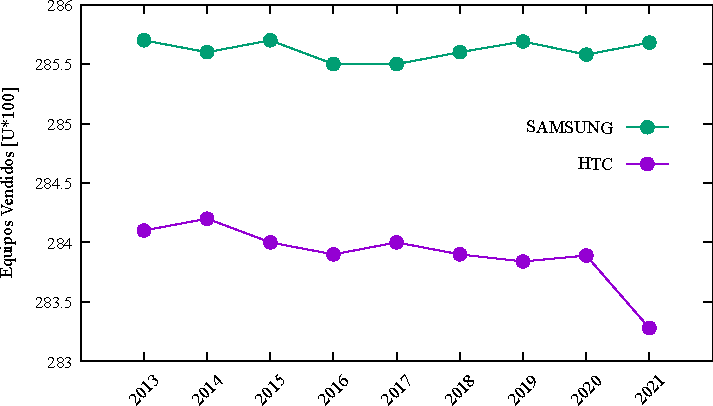
\includegraphics[width=0.7\linewidth]{images/Lecture_1h}
            \caption{Equipos celulares vendidos por las compañías SAMSUNG y HTC en el periodo 2013-2021. }
            \label{fig:lecture1h}
        \end{figure}
      \end{frame}

      \begin{frame}{Gráficos estadístico. Ejemplo}
        \begin{figure}
            \centering
            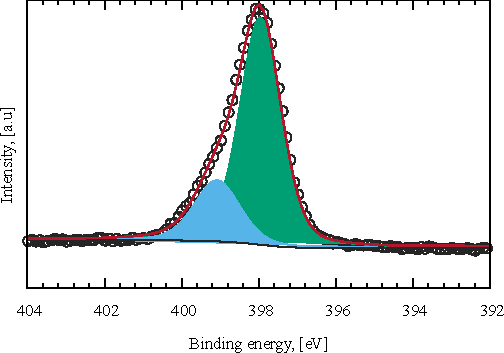
\includegraphics[width=0.7\linewidth]{images/Lecture_1i}
            \caption{Espectro XPS de una muestra de pyridina. }
            \label{fig:lecture1i}
        \end{figure}

      \end{frame}
      \subsubsection*{Tipos de gráficos estadístico}

      \begin{frame}{Gráficos estadístico. Representación de tronco y hoja}
          Las gráficas de tallos y hojas son una forma rápida de obtener la representación visual informativa
de un conjunto de datos.

          Es un método exploratorio, que permite visualizar la distribución de los datos de una manera gráfica, pero sin llegar a elaborar un gráfico.

          Pasos para construir una gráfica de tallos y hojas
          \begin{enumerate}
              \item Seleccione uno o más de los primeros dígitos para los valores de tallo. Los segundos dígitos se convierten en hojas.
              \item Enumere los posibles valores de tallos en una columna vertical.
              \item Anote la hoja para cada observación junto al valor de tallo.
              \item Indique las unidades para tallos y hojas en algún lugar de la gráfica.
          \end{enumerate}



      \end{frame}

      \begin{frame}{Gráficos estadístico. Representación de tronco y hoja}
          Pasos para construir una gráfica de tallos y hojas
          \begin{enumerate}
              \item Seleccione uno o más de los primeros dígitos para los valores de tallo. Los segundos dígitos se convierten en hojas.
              \item Enumere los posibles valores de tallos en una columna vertical.
              \item Anote la hoja para cada observación junto al valor de tallo.
              \item Indique las unidades para tallos y hojas en algún lugar de la gráfica.
          \end{enumerate}

          Tomemos la siguiente tabla como ejemplo:
          \begin{table}[!h]
              \centering
              \begin{tabular}{|c|c|c|c|c|}
                  \hline
                  5.0 & 5.5 & 6.2 & 6.5 & 6.6 \\
                  \hline
                  6.7 & 6.7 & 7.1 & 7.3 & 7.7 \\
                  \hline
                  7.7 & 7.9 & 8.3 & 8.5 & 8.5 \\
                  \hline
                  8.8 & 8.8 & 8.9 & 9.0 & 9.1 \\
                  \hline
                  9.1 & 9.1 & 9.2 & 9.3 & 9.3 \\
                  \hline
              \end{tabular}
          \end{table}
      \end{frame}

      \begin{frame}{Gráficos estadístico. Representación de tronco y hoja}
         % \centering
        5|0 5\\
        6| 2 5 6 7 7\\
        7|1 3 7 7 9\\
        8| 3 5 5 8 8 9\\
        9|0 1 1 2 3 3\\
      \end{frame}

      \begin{frame}{Gráficos estadístico. Histogramas. Tabla de Frecuencias.}
          Para las distribuciones de frecuencias la representación gráfica más común es el histograma.
          \begin{block}{Frecuencia y Frecuencia relativa}
              Considérense datos compuestos de observaciones de una variable discreta x. La\textbf{ frecuencia} de cualquier valor x particular es el número de veces que ocurre un valor en el conjunto de datos. La \textbf{frecuencia relativa} de un valor es la fracción o proporción de veces que
ocurre el valor. El cual se obtiene dividiendo la \textbf{frecuencia relativa} de un valor entre el \textbf{número de observaciones en el conjunto de datos}.

          \end{block}
      \end{frame}

      \begin{frame}{Gráficos estadístico. Histogramas. Tabla de Frecuencias.}

        \begin{block}{Ejemplo}
          Supóngase, por ejemplo, que un conjunto de datos se compone de 200 observaciones y x representa el número de cursos que un estudiante está tomando en un cuatrimestre. Si 70 de estos valores x es igual a 3, entonces:

          \pause
          frecuencia del valor 3 es 70 veces, o dicho de otro modo, hay 70 estudiantes que tomaron 3 materias.
          \pause
          $$FR =\dfrac{70}{200}= 0.35$$

          Si se multiplica una frecuencia relativa por 100 se obtiene un 35\%.\\
          \pause
          Una \textbf{distribución de frecuencia} es una \textbf{tabla de las frecuencias} o de las frecuencias relativas, o de ambas.
       \end{block}
      \end{frame}

      \begin{frame}{Gráficos estadístico. Histogramas}
        \pause
        \begin{block}{Construcción de un histograma}
          En primer lugar, se determina la frecuencia y la frecuencia relativa de cada valor x.
Luego se marcan los valores x posibles en una escala horizontal. Sobre cada valor, se
traza un rectángulo cuya altura es la frecuencia relativa o alternativamente, la frecuencia de dicho valor.
        \end{block}
        \begin{figure}
            \centering
            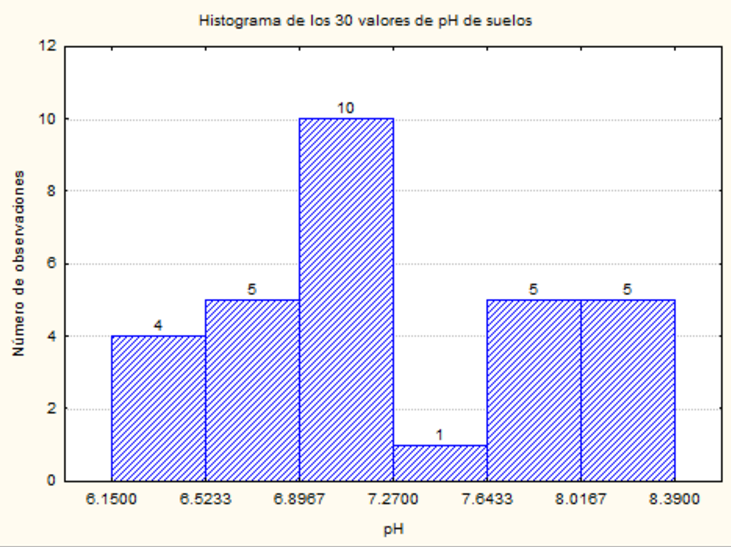
\includegraphics[width=0.5\linewidth]{images/histograma}

            \label{fig:histograma}
        \end{figure}
      \end{frame}

       \begin{frame}{Gráficos estadístico. Formas de los Histogramas }
         \begin{figure}
             \centering
             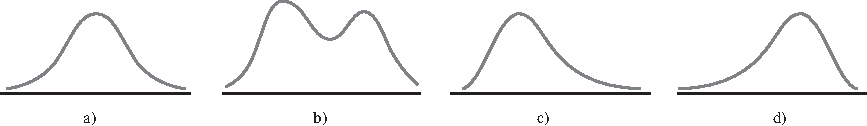
\includegraphics[width=0.7\linewidth]{images/formas_histograma}
             \label{fig:formashistograma}
         \end{figure}
         \pause
         \begin{figure}
             \centering
             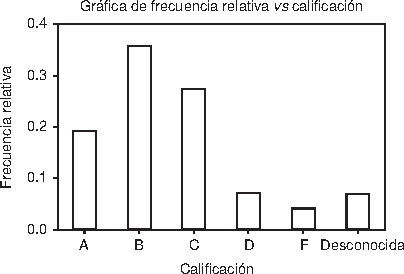
\includegraphics[width=0.7\linewidth]{images/cualitativo_histograma}
             \caption{}
             \label{fig:cualitativohistograma}
         \end{figure}


      \end{frame}




      \begin{frame}{Gráficos estadístico. Gráficos de barras}
          Un tipo de gráfico muy parecido al histograma es la gráfica de barras.   A diferencia del histograma, no es necesario tener una escala horizontal continua. Se pueden colocar varias series, por lo que deben seleccionarse colores y anchos de las barras que nos permitan diferenciarlos.
          \begin{figure}
              \centering
              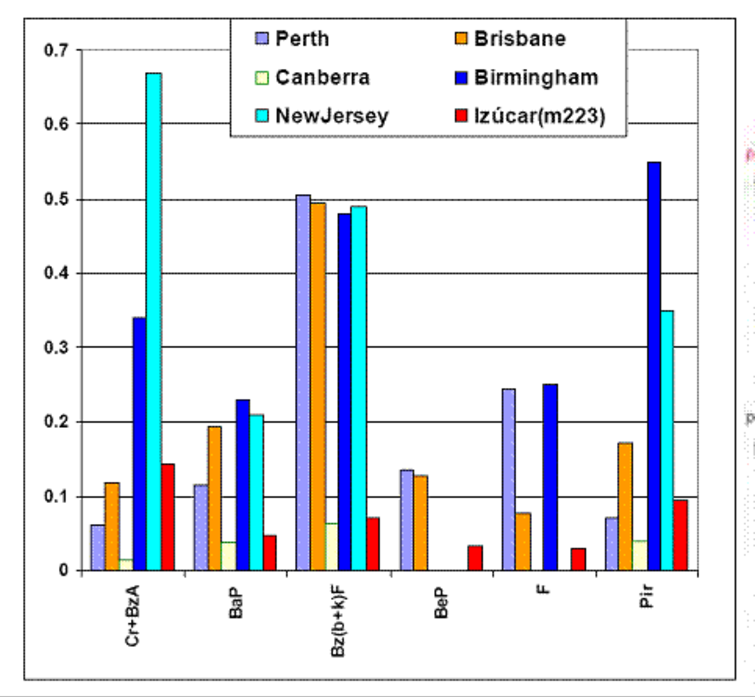
\includegraphics[width=0.5\linewidth]{images/graficos_barra1}
              \label{fig:graficosbarra1}
          \end{figure}
      \end{frame}

      \begin{frame}{Gráficos estadístico. Gráficos de barras}

        \begin{figure}
          \centering
          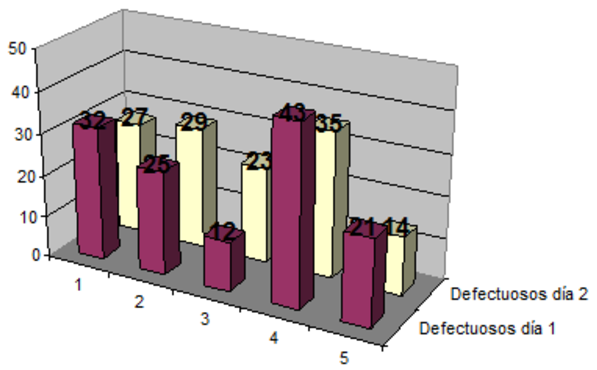
\includegraphics[width=0.7\linewidth]{images/graficos_barra2}
          \caption{Gáfico de barras 3D.}
          \label{fig:graficosbarra2}
        \end{figure}
      \end{frame}


      \begin{frame}{Gráficos estadístico. Gráficos de barras}
        \begin{figure}
          \centering
          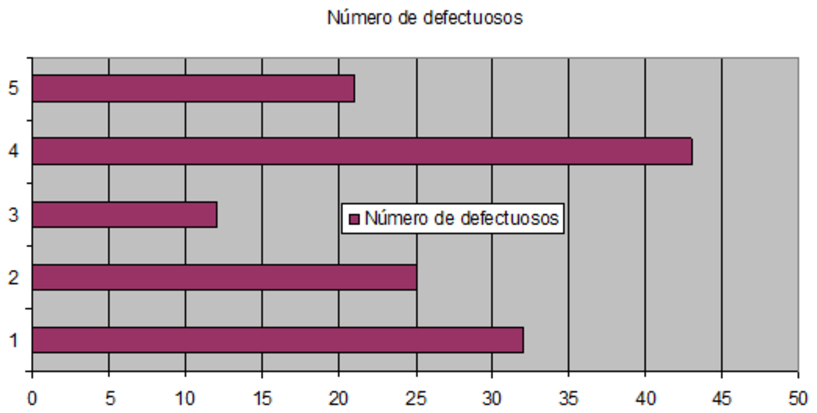
\includegraphics[width=0.7\linewidth]{images/graficos_barra3}
          \caption{Gáfico de barras horizontal.}
          \label{fig:graficosbarra3}
        \end{figure}
      \end{frame}

      \begin{frame}{Gráficos estadístico. Gráfica de lineas}
          Cuando los datos se relacionan entre sí, es decir, existe cierta continuidad entre las observaciones (como por ejemplo el crecimiento poblacional, la evolución del peso de una persona, las variaciones presentadas en la medición realizada en algún experimento con determinada temporalidad) se pueden utilizar las gráficas de líneas.
          \begin{figure}
              \centering
              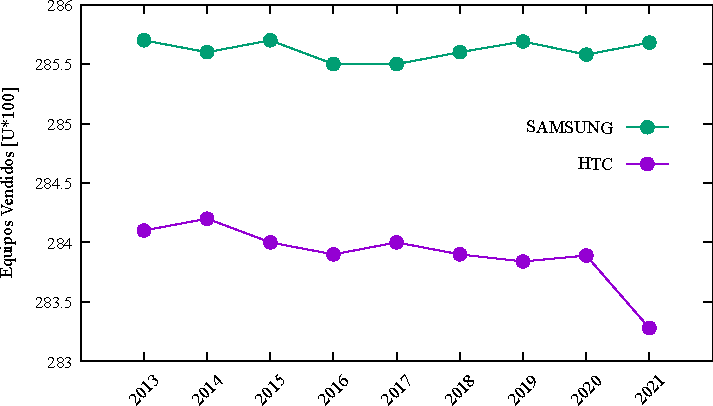
\includegraphics[width=0.6\linewidth]{images/Lecture_1h}
              \label{fig:lecture1hh}
          \end{figure}

      \end{frame}

       \begin{frame}{Gráficos estadístico. Polígono de frecuencias}
          En el polígono de frecuencias se añaden dos clases con frecuencias cero: una antes de la primera clase con datos y otra después de la última. El resultado es que se "sujeta" la línea por ambos extremos al eje horizontal y lo que podría ser una línea separada del eje se convierte, junto con éste, en un polígono.
         \begin{figure}
             \centering
             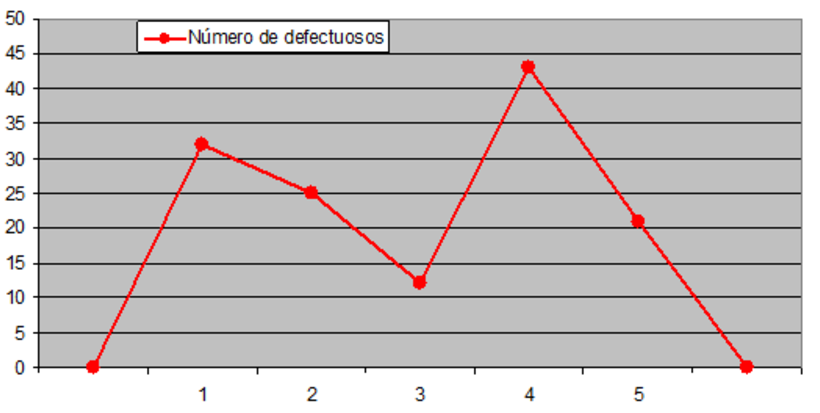
\includegraphics[width=0.6\linewidth]{images/graficos_poligonodef}
             \label{fig:graficospoligonodef}
         \end{figure}

      \end{frame}

      \begin{frame}{Gráficos estadístico. Gráfico de frecuencias acumuladas u ojiva}
          Su objetivo, al igual que el histograma y el polígono de frecuencias es representar distribuciones de frecuencias de variables cuantitativas, pero sólo para frecuencias acumuladas. No se utilizan barras en su confección, sino segmentos de recta.
          \begin{figure}
              \centering
              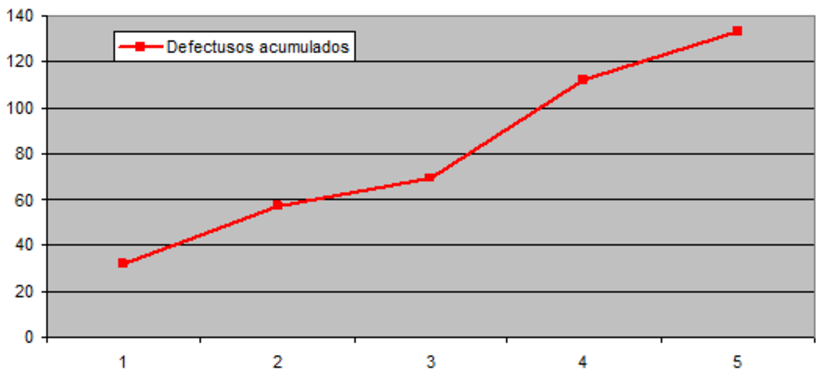
\includegraphics[width=0.7\linewidth]{images/graficos_ojiva}
              \label{fig:graficosojiva}
          \end{figure}
      \end{frame}

      \begin{frame}{Gráficos estadístico. Gráfica de pastel}
        Cuando se desea resaltar las proporciones que representan algunos subconjuntos con respecto al total, son útiles las gráficas de pastel.
        \begin{figure}
            \centering
            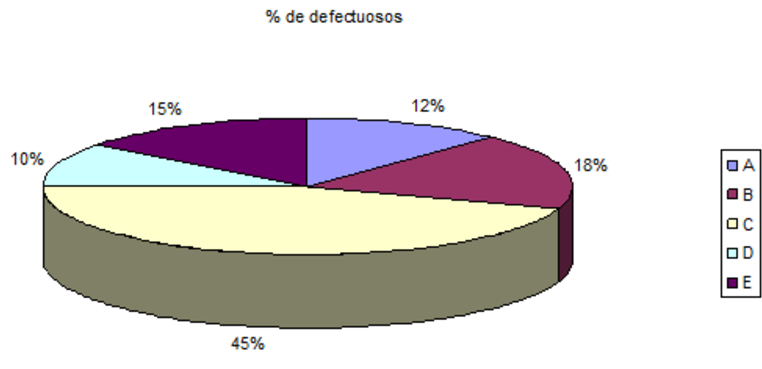
\includegraphics[width=0.7\linewidth]{images/graficos_pastel}
            \label{fig:graficospastel}
        \end{figure}
      \end{frame}

      \begin{frame}{Gráficos estadístico. Gráficas de dispersión}
        Se utilizan mucho para evaluar datos experimentales. Se representan los valores de una variable dependiente, en el eje de las ordenadas, contra los valores de las variables independientes que corresponden, en el eje de las ordenadas. Esto nos permite evaluar tendencias, correlaciones, etc.
        \begin{figure}
            \centering
            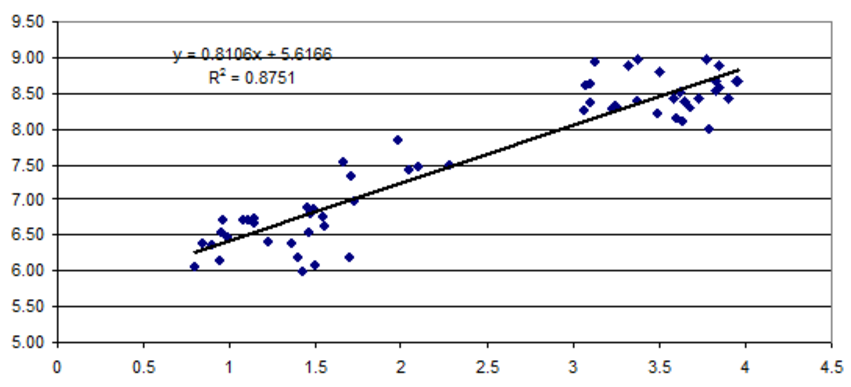
\includegraphics[width=0.7\linewidth]{images/graficos_dispersion}
            \label{fig:graficosdispersion}
        \end{figure}
      \end{frame}


    \begin{frame}
      \centering
      \textit{\textbf{ \huge  TO BE CONTINUE}}
    \end{frame}


\end{document}